\section{Motivation}
The motivation of this experiment is to determine the magnetic moment caused by the spin of a free electron and their gyromagnetic ratio.
Diphenylpikrylhydracyl is a sample which offers free electrons. Methods of high frequency spectroscopy are used for this purpose:
The experimental conditions are varied until a resonance absorption of the electrons occurs. With the resonance condition it is possible
to determine the magnetic moment.
\section{Theory}
Electrons without orbital angular momentum still have a magnetic moment. This is not compatible with classical physics
and can only be explained by quantum physics.
According to quantum physics electrons have a kind of inner orbital angular momentum, called spin. \\
\subsection{Realtionship between magnetic moment and orbital angular momentum}
First of all, based on the consideration that the
wave function for an atom in the one-electron approximation can be represented as
\begin{equation}
  \psi_{n,l,m}(r,\vartheta,\varphi)=R_{n,l}(r)\uptheta_{l,m}(\vartheta)\upphi(\varphi)=\frac{R_{n,l}(r)\uptheta_{l,m}\symup{e}^{im\varphi}}{\sqrt{2\pi}},
\end{equation}
a relationship between the orbital angular momentum
and the magnetic moment can be found.
\begin{equation}
  \mu_B=-\frac{e_0\hbar m}{2m_0}
\end{equation}
$m\hbar$ is the orbital angular momentum and $\mu_B$ is the product of the natural constants, called Bohr Magneton.
\subsection{Splitting of the energy levels in an external magnetic field}
If an external magnetic field is applied, the energy levels of an eletron are split (Zeeman Effect).
The spin quantum number is calculated as
then according to
\begin{equation}
  2s+1=2
\end{equation}
This is due to the fact that the components of a vector are at most equal to their
amount, the Orientation quantum number $m$ only assume the following values:
\begin{equation}
  m=0,\pm1,\pm2,...,\pm l
\end{equation}
So there are only $2l+1$ settings for the Orientation quantum number $m$, where $l$ is the orbital angular momentum.
Therefore, the following relationship applies to the Z-component of the spin:
\begin{equation}
  S_Z=m_s\hbar=\pm\frac{\hbar}{2}.
\end{equation}
The magnetic moment $\mu$ of the spin is then
\begin{equation}
  \mu_{S_Z}=-\frac{g\cdot\mu_B}{2}.
\end{equation}
$g$ is referred to as the gyromagnetic ratio and may assume a value other than 1.
\subsection{Electron Paramagnetic Resonance}
The Electron Paramagnetic Resonance method is used to determine the gyromagnetic ratio $g$.
This ratio describes how the spin-caused magnetic moment differs from the magnetic moment caused by the orbital angular momentum.
With an external magnetic field, the energy of a free electron is converted into two sub-levels,
where the energy difference between the two levels is
\begin{equation}
  \increment E=g\mu_B B.
  \label{eq:ediff}
\end{equation}
If now energy, which corresponds to the energy difference $\increment E$,
is supplied to the system in form of light quanta, then \ref{eq:ediff} results to
\begin{equation}
  h\nu=g\mu_B B.
  \label{eq:gyro}
\end{equation}
The electrons on the lower energy level are now able to absorb the energy, switch their spin and therefore reach the higher energy level. This
is called Electron Paramagnetic Resonance. The
excited electrons do not remain on that higher level, but dispense the additional energy in complicated ways to their surroundings.
\begin{figure}
  \centering
  \begin{circuitikz}
    \draw[->,brown] (1,2)--(1,0);
    \draw[->,brown] (2,2)--(2,0);
    \draw[->,brown] (3,2)--(3,0);
    \draw[->,brown] (0,2)--(0,0);
    \node[brown] at (3.3,0){$H$};
    \draw[->] (-1,0)--(-1,2);
    \draw (-1.1,1.5)--(-0.9,1.5);
    \draw (-1.1,0.7)--(-0.9,0.7);
    \node at (-1.3,2.3){$E$};
    \node[font=\small] at (-2.1,1.5){$E_{0}+\frac{1}{2}\text{g\mu}_\text{B} \text{H}$};
    \node[font=\small] at (-2.1,0.7){$E_{0}-\frac{1}{2}\text{g\mu}_\text{B} \text{H}$};
    \draw[->] (-0.7,0.7)--(-0.7,1.5);
    \draw[decorate,decoration={brace,amplitude=6pt}](-0.5,1.5)--(-0.5,0.7);
    \node[font=\small] at (0.5,1.1){$\increment E=h\nu$};
  \end{circuitikz}
  \caption{Energy level of free electrons split into two by an external magnetic field $H$. $\increment E$ can be modified by varying $H$.}
  \label{}
\end{figure}
It is possible to measure this effect by placing a sample into a coil of a bridge circuit and inducing a homogeneous magnetic field by a Helmholtz coil.
If now a high frequency voltage produces a high frequency magnetic field in the sample-coil, the transition shown in figure \ref{} is induced which causes a change of
the magnetism of the sample. As a consequence this change of magnetism becomes visible as a change of the bridge voltage, that has been balanced without the homogenous magnetic beforehand. \\ \\ \noindent
The magnetic field of a Helmholtz coil can be determined with
\begin{equation}
  B(I)=\frac{8\mu_0 n I}{\sqrt{125}\cdot r}
  \label{eq:mfield}
\end{equation}
where $\mu_0$ is the vacuum permeability. A high-frequency voltage is applied to the bridge circuit.
When the bridge voltage is measured as a function of a changing current (the one inducing the homogenous magnetic field in the Helmholtz coil) one of two possible graphs shown in figure \ref{two}
can be seen on a connected oscilloscope.
\begin{figure}[H]
  \centering
  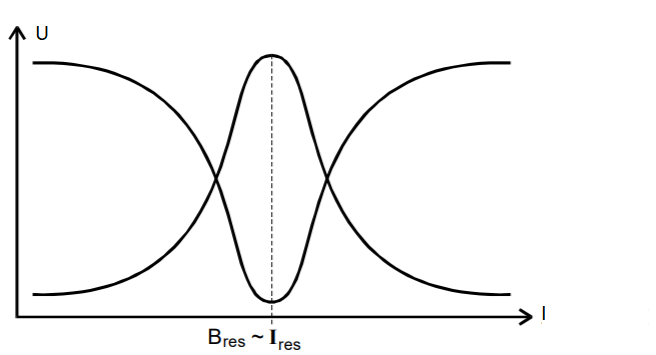
\includegraphics[scale=0.75]{two.png}
  \caption{Possible Measurements of the Electron Paramagnetic Resonance. \cite{1}} \label{two}
\end{figure}
